\section{Change Request}
For this Software Maintenance report document, i have chosen to work with the feature called \textit{Tool Palette.}
The refactoring of the code will be done in a group consisting of 5 students total, including myself. We have each choosen af feacture to reactore doing the course of this project.

The infomation we have gotten on the different features are only a short descriptive text, with the name of the feature. For my chosen feature the text is the following: \textit{Tool Palette - Display, Drag and Drop.}
With this feature name i can with some analysis and implementation of the given code I can figure out what i have to reactore within my feature.
As I am working with the feacture called \textit{Tool Palette,} I will assume the whole of the tool palette is within my feacture. The \textit{Tool Palette} after inspection looks to contain
tool sections, where it has different tools that one can select within these sections.

As part of the project we have made individual User Stories for our chosen feature. My User Story are the following:

\textbf{Drag and Drop}

The \textit{Drag/Drop} user story outlines a feature, that is designed to enable users of the program to customize their workspace within the program itself.
It allows the user to drag and drop different sections of the toolbar, to a location of their choosing.
By allowing the user to customize their workspace, it can impove their work efficiency, but have their most used tools and options within easy reach.

\begin{figure}[htbp]
    \centering
    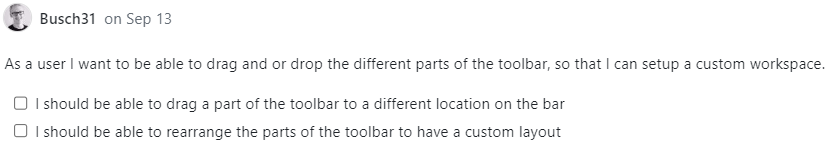
\includegraphics[width=\linewidth]{pic/Tool_palette_Drag_and_drop.png}
    \caption{User Story for Drag and Drop.}
    \label{fig:tool-palette-drag-drop}
\end{figure}

\textbf{Display}

The \textit{Display} user story outlines a feature, that is designed to enable the users to show or hide different sections of the toolbar to their liking.
Thereby allowing the users to hide or show only the tool section, that are relevant to their current task. It will also give the user less clutter on their screen doing their work.


\begin{figure}[htbp]
    \centering
    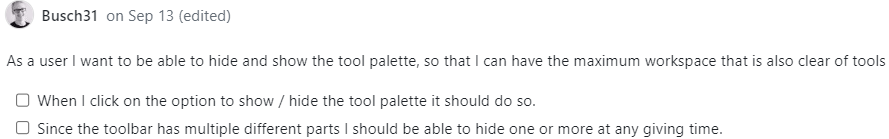
\includegraphics[width=\linewidth]{pic/Tool_palette_Display.png}
    \caption{User Story for Display.}
    \label{fig:tool-palette-display}
\end{figure}

To successfully complete the refactoring, the following steps should be undertaken by us as a group:
\begin{itemize}
    \item Learn the feature scope of our different features within the codebase by doing a concept location to identify the relevant classes and tools.
    \item Evaluate the estimated impact of the refactoring on each developers features to anticipate any potential overlaps or conflicts our different features might have or could have.
    \item Understand the sections of code that require refactoring by identifying it with code smells.
    \item Carry out the refactoring while trying to minimize any unintended cascading changes that could happen with refactoring.
    \item Verify the changes after refactoring to ensure they achieve the desired outcome and that the primary function of the code is still maintained.
\end{itemize}

Besides having to do this refactoring, we as a group also have to setup continuous integration,
thereby ensuring that any code is tested and verified before it is merged into the main branch.
